\textbf{Входные параметры:}
 
 Parent1 --- первый родитель;
 
 Parent2 --- второй родитель;
 
 VHML\_ResultVector --- потомок;
 
 VHML\_N --- размер векторов Parent1, Parent2 и VHML\_ResultVector.

\textbf{Возвращаемое значение:}

 Отсутствует.
 
\begin{align*}
&Crossover \left( \overline{Parent}^1, \overline{Parent}^2, DataOfCros\right) = \overline{Offspring};\\
& \overline{Offspring}_i=Random\left( \left\lbrace \overline{Parent}^1_i;\overline{Parent}^2_i\right\rbrace \right), i=\overline{1,n} ;\nonumber\\
&\overline{Offspring}\in X.\nonumber
\end{align*}

$ DataOfCros $ не содержит каких-либо параметров относительно данного типа скрещивания.

\textbf{Пример.} Двухточечное скрещивание показано на рисунке:

\begin{figure} [h]
  \center
  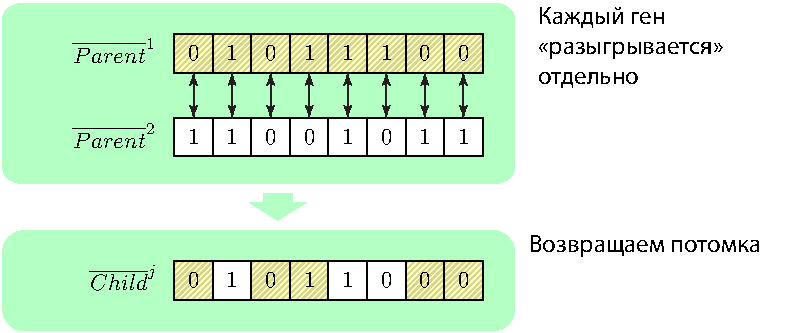
\includegraphics [scale=0.8] {HML_UniformCrossover_Sheme}
  \caption{Механизм работы равномерного скрещивания} 
  \label{img:HML_UniformCrossover_Sheme}  
\end{figure}